\subsection{Кинематика твёрдого тела}

\subsubsection*{3.24}


\begin{wrapfigure}{r}{0.35\textwidth}
  \begin{center}
        \vspace{-10 mm}
        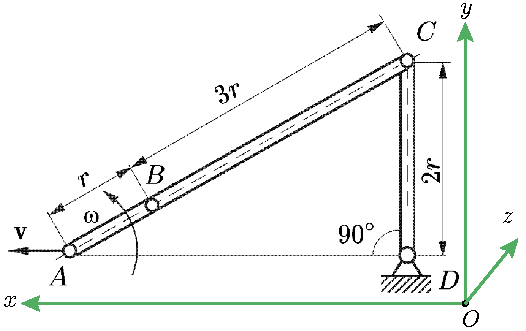
\includegraphics[width=0.9\linewidth]{img/3_24.pdf}
  \end{center}
    \caption{К задаче 3.24.}
    %\label{fig:}
\end{wrapfigure}


Запишем $\vc{v}_B$, выбрав в качестве полюса точку $A$ и точку $C$.
\begin{align}
\label{vb}
    \vc{v}_{B} = \vc{\omega} \times \vv{AB} + \vc{v} = \vc{v}_{C} + \vc{\omega}_{BC} \times \vv{CB},
\end{align}
или, расписав по координатам,
$$
\underbrace{\begin{pmatrix}
        0 \\ 0 \\ \omega
    \end{pmatrix} \times \begin{pmatrix}
        - r \cos \alpha \\
        r \sin \alpha \\
        0
    \end{pmatrix}}_{\vc{\omega} \times \vv{AB}}
    + \begin{pmatrix}
        v \\
        0 \\
        0
    \end{pmatrix} =
    \begin{pmatrix}
        v_C \\
        0 \\
        0
    \end{pmatrix} +
    \begin{pmatrix}
        0 \\
        0 \\
        \omega_{BC}
    \end{pmatrix} \times
    \begin{pmatrix}
        3r \cos \alpha \\
        -3r \sin \alpha \\
        0
    \end{pmatrix},
$$
получим два содержательных уравнения
$$
    \left.\begin{aligned}
        -r\omega \sin \alpha + v &= v_c + 3r \omega_{BC} \sin \alpha \\
        -r\omega \cos \alpha  + 0&= 0 \;\, + 3r \omega_{BC} \cos \alpha
    \end{aligned}\right\}
    \hspace{0.5cm} \Rightarrow \hspace{0.5cm} 
    \boxed{
    \vc{\omega}_{BC} = -\frac{\vc{\omega}}{3},
    \hspace{0.5cm} \vc{v}_C = \vc{v}.
    }
$$

\phantom{42}    

Для поиска $\vc{\mathrm{w}}_C$, запишем условия жёсткости стержней $BC$ и $CD$. Дифференцируя по времени, получим
\begin{equation}
\label{eq_12}
        \left.\begin{aligned}
            \vc{v}_B \cdot \vv{BC} &= \vc{v}_C \cdot \vv{BC}; \\
             \vc{v}_C \cdot \vv{DC} &= 0.
        \end{aligned}\right\}
    \hspace{0.25cm} \overset{d / dt}{\Rightarrow}  \hspace{0.25cm} 
        \left\{\begin{aligned}
        \vc{\mathrm{w}}_B \cdot \vv{BC} + \vc{v}_B \cdot \dot{\vv{BC}} &=
        \vc{\mathrm{w}}_C \cdot \vv{BC} + \vc{v}_C \cdot \dot{\vv{BC}}; \\
        \vc{\mathrm{w}}_C \cdot \vv{DC} + \vc{v}_C \cdot \dot{\vv{DC}} &= 0.
        \end{aligned}\right.
\end{equation}
Выразим $\vc{\mathrm{w}}_B$ из уравнения Ривальса:
$$
    \vc{\mathrm{w}}_B = \underbrace{\vc{\mathrm{w}}_A}_{0} + \underbrace{\dot{\omega}_{AB} \times \vv{AB}}_{0} +
    \,
     \vc{\omega} \times \left(
        \vc{\omega} \times \vv{AB}
    \right) = \begin{pmatrix}
        0 \\ 0 \\ \omega
    \end{pmatrix} 
    \begin{pmatrix}
        -r\omega\sin\alpha \\
        -r\omega\cos\alpha \\
        0
    \end{pmatrix} = \begin{pmatrix}
        r\omega^2 \cos \alpha \\
        -r\omega^2 \sin \alpha \\
        0
    \end{pmatrix}.
$$
В первом уравнении \eqref{eq_12}, зная $\dot{\vv{BC}} = \vc{\omega}_{BC} \times \vv{BC} = (\omega r \sin \alpha,\; \omega r \cos \alpha,\; 0)\T$ и $\vc{v}_B$ из \eqref{vb}, получим
\begin{equation}
    \label{eqI}
    \vc{\mathrm{w}}_C \cdot \vv{BC} = - 4 \omega^2 r^2.
\end{equation}
Во втором уравнении \eqref{eq_12}, зная $\dot{\vv{DC}} = \vc{\omega}_{DC} \times \vv{DC} = \vc{v}_C$, получим
\begin{equation}
    \label{eq2}
    \vc{\mathrm{w}}_C \cdot \vv{DC} = -v^2.
\end{equation}
Из \eqref{eq2}, мы знаем $(\vc{\mathrm{w}}_C)_y$, расписав в \eqref{eqI} проекцию на $BC$ покоординатно, получим
$$
    \left.\begin{aligned}
        -4 \omega^2 r^2 &= 3r (-{\mathrm{w}}_{Cx} \cos \alpha + {\mathrm{w}}_{Cy} \sin \alpha); \\
        {\mathrm{w}}_{Cy} &= -{v^2}/{2r} .
    \end{aligned}\right\}
    \hspace{0.5cm} \Rightarrow \hspace{0.5cm} 
        \vc{\mathrm{w}}_C = 
        \begin{pmatrix}
            \mathrm{w}_{Cx} \\
            \mathrm{w}_{Cy} \\
            0
        \end{pmatrix},
    \hspace{0.25cm} \text{где} \hspace{0.25cm} 
    \mathrm{w}_{Cx} = \frac{8\sqrt{3}}{9} \omega^2 r - \frac{\sqrt{3}}{6} \frac{v^2}{r}, \;
    \mathrm{w}_{Cy} = -\frac{v^2}{2r}.
$$
Собственно\footnote{
    Вычисления доступны здесь.
}, $\|\vc{\mathrm{w}}_C\|^2 = \frac{64}{27}\omega^{4} r^{2} - \frac{8 }{9}\omega^{2} v^{2} + \frac{1}{3} {v^{4}}/{ r^{2}} $.


%%%%%%%%%%%%%%%%%%%%%%%%%%%%%%%%%%%%%%%%%%%%%%%%%%%%%%%%%%%%%%%%%%%%%%%%%%%%%%%%%%%


\subsubsection*{4.4}



Запишем в координатах $\omega_1$ и $\omega_2$.
$$
    \vc{\omega}_1 = \begin{pmatrix}
        0 \\ \omega_1 \sin \theta \\ \omega_1 \cos \theta
    \end{pmatrix};
    \hspace{0.5cm} 
    \vc{\omega}_2 = \begin{pmatrix}
        0 \\ 0 \\ \omega_2
    \end{pmatrix}.
$$

Так как оси $\omega_1$  и $\omega_2$ пересекаются, угловая скорость и угловое ускорение можно найти, как
$$
    \vc{\omega} = \vc{\omega}_1 + \vc{\omega}_2 = \begin{pmatrix}
        0 \\ \omega_1 \sin \theta \\ \omega_2 + \omega_1 \cos \theta
    \end{pmatrix},
    \hspace{1cm} 
    \vc{\varepsilon} = \vc{\omega}_1 \times \vc{\omega}_2 = \begin{pmatrix}
        \omega_1 \omega_2 \sin \theta \\ 0 \\ 0
    \end{pmatrix},
$$
что очень похоже на правду.

\begin{center}
    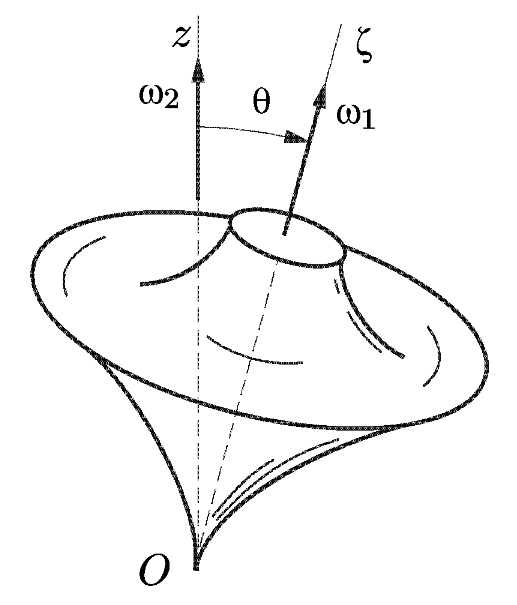
\includegraphics[width=0.2\textwidth]{img/4_4.png}
    \hspace{3cm} 
    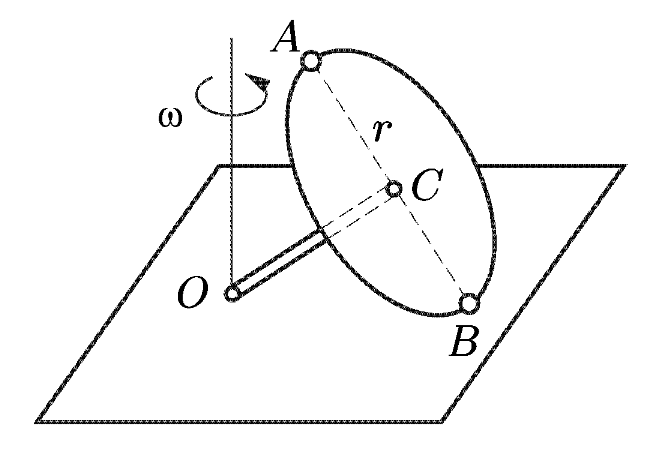
\includegraphics[width=0.3\textwidth]{img/4_10.png}\\
    Рисунки к задачам 4.4 и 4.10.
\end{center}

%%%%%%%%%%%%%%%%%%%%%%%%%%%%%%%%%%%%%%%%%%%%%%%%%%%%%%%%%%%%%%%%%%%%%%%%%%%%%%%%%%%
\subsubsection*{4.10}

Запишем $\vc{v}_c$, как результат движения стержня и диска. Пусть $\Omega$ -- угловая скорость вращения диска, $\parallel OB$.
$$
    \vc{v}_C = \vc{\Omega} \times \vv{BC} = \vc{\Omega} \times \vv{OC} =
    \vc{\omega} \times \vv{OC}.
$$
Другими словами, в координатной записи,
$$
    \begin{pmatrix}
        \Omega \\ 0 \\ 0
    \end{pmatrix} \times \begin{pmatrix}
        3 \\ \sqrt{3} \\ 0
    \end{pmatrix} \frac{r}{2}  = \begin{pmatrix}
        0 \\ \omega \\ 0
    \end{pmatrix} \times \begin{pmatrix}
        3 \\ \sqrt{3} \\ 0
    \end{pmatrix} \frac{r}{2}
    \hspace{0.5cm} \Rightarrow \hspace{0.5cm} 
    \boxed{\Omega = - \sqrt{3} \omega}.
$$
Угловое ускорение стержня найдём, как движение в СО стержня,
$$
    \vc{\varepsilon}^a = \vc{\varepsilon} + \vc{\varepsilon}^r + \vc{\omega} \times \vc{\Omega} =
    \begin{pmatrix}
        0 \\ \varepsilon \\ 0
    \end{pmatrix} +
    \begin{pmatrix}
        -\sqrt{3}\varepsilon \\ - \varepsilon \\ 0
    \end{pmatrix} +
    \begin{pmatrix}
        0 \\0 \\ \sqrt{3} \omega^2
    \end{pmatrix} = \begin{pmatrix}
        - \sqrt{3} \varepsilon \\ 0\\ \sqrt{3} \omega^2
    \end{pmatrix}
    \hspace{0.5cm} \Rightarrow \hspace{0.5cm} 
    \boxed{\varepsilon^a = \sqrt{3\left(\varepsilon^2 + \omega^4\right)}},
$$
где
$$
    \vc{\varepsilon}^r = \vc{\dot{\omega}} = \frac{d}{dt} \left(\vc{\Omega} - \vc{\omega}\right) = \frac{d}{dt} \begin{pmatrix}
        - \sqrt{3} \omega \\ -\omega \\ 0
    \end{pmatrix} = \begin{pmatrix}
        - \sqrt{3} \varepsilon \\ - \varepsilon \\ 0
    \end{pmatrix}.
$$
Теперь, из сложения ускорений,
$$
    \vc{\mathrm{w}}^a = \underbrace{\vc{\mathrm{w}}_0 + \vc{\varepsilon} \times \vc{r} + \vc{\omega} \times \vc{\omega} \times \vc{r}}_{\vc{\mathrm{w}}^e} + \underbrace{2 \vc{\omega} \times \vc{v}^r}_{\vc{\mathrm{w}}^c} + \vc{\mathrm{w}}^r,
$$
найдём $\vc{\mathrm{w}}_B^a$:
$$
    \vc{\mathrm{w}}_B^a = \vc{0} + \vc{\varepsilon} \times \vv{OB} + \vc{\omega} \times \left(
        \vc{\omega} \times \vv{OB}
    \right) + 2 \vc{\omega} \times \left(- \vc{\omega} \times \vv{OB} \right) + \vc{\mathrm{w}}^r_B.
$$
Теперь найдём $\vc{\mathrm{w}}^r_B$, как
$$
    \vc{\mathrm{w}}^r_B = \vc{\mathrm{w}}_{\tau}^r + \vc{\mathrm{w}}_n^r =
    - \varepsilon r \begin{pmatrix}
        \sqrt{3} \\ 1 \\ 0
    \end{pmatrix} \times \begin{pmatrix}
        2 \\ 0 \\ 0
    \end{pmatrix} + \omega^2 \frac{1}{2} \begin{pmatrix}
        - r \\ r \sqrt{3} \\ 0
    \end{pmatrix}.
$$
Подставляя, дойдём до
$$
    \boxed{\vc{\mathrm{w}}_B^a = \begin{pmatrix}
        0 \\ 2 \sqrt{3} \omega^2 r \\ 0
    \end{pmatrix}}
    \hspace{0.5cm} \Rightarrow \hspace{0.5cm} 
    \|\vc{\mathrm{w}}^a_B\| = 2 \sqrt{3} \omega^2 r,
$$
что, достаточно, логично.

Аналогично найдём $\vc{\mathrm{w}}^a_A$:
$$
    \vc{\mathrm{w}}^a_A = \vc{0}  + \begin{pmatrix}
        0 \\ \varepsilon \\ 0 
    \end{pmatrix} \times \begin{pmatrix}
        1 \\ \sqrt{3} \\ 0
    \end{pmatrix} r - \begin{pmatrix}
        0 \\ \omega \\ 0
    \end{pmatrix} \times
    \begin{pmatrix}
        0 \\ \omega \\ 0
    \end{pmatrix} \times
    \begin{pmatrix}
        1 \\ \sqrt{3} \\ 0
    \end{pmatrix} r +
    2 \omega^2 r \begin{pmatrix}
        1 \\ -\sqrt{3} \\ 0
    \end{pmatrix} - \varepsilon r \begin{pmatrix}
        0 \\ 0 \\ 2
    \end{pmatrix},
    \hspace{0.2cm} \Rightarrow \hspace{0.2cm} 
    \boxed{\vc{\mathrm{w}}^a_A = r \begin{pmatrix}
        3 \omega^2 \\ 2 \sqrt{3} \omega^2 \\ - 3 \varepsilon 
    \end{pmatrix}}.
$$
И найдём норму ускорения точки $A$
$$
    \|\vc{\mathrm{w}}_A^a\| = \sqrt{21 \omega^4 r^2 + 9 \varepsilon^2 r^2}.
$$


%%%%%%%%%%%%%%%%%%%%%%%%%%%%%%%%%%%%%%%%%%%%%%%%%%%%%%%%%%%%%%%%%%%%%%%%%%%%%%%%%%%
\subsubsection*{4.12}

\begin{wrapfigure}{r}{0.35\textwidth}
  \begin{center}
        \vspace{-14 mm}
        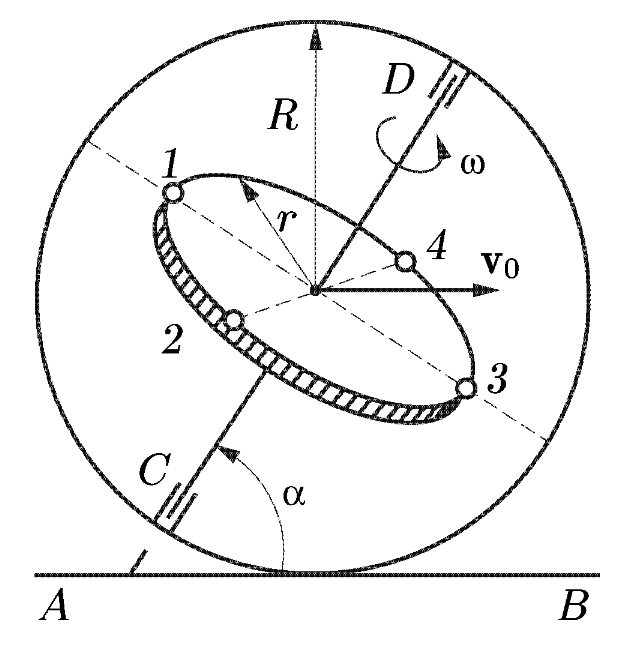
\includegraphics[width=0.8\linewidth]{img/4_12.png}
  \end{center}
    % \caption*{К задаче 4.12}
    %\label{fig:}
\end{wrapfigure}


Расмотрим движение интересных нам точек, как движение в СО обруча, с
$$
    \vc{v}^e = \vc{v} = \begin{pmatrix}
        v \\ 0\\ 0
    \end{pmatrix};
    \hspace{0.5cm} 
    \vc{\omega}^e = \begin{pmatrix}
        0 \\ 0 \\ - v / R
    \end{pmatrix};
    \hspace{0.5cm} \vc{\mathrm{w}}^e = \vc{0};
    \hspace{0.5cm} \vc{\varepsilon}^e = \vc{0}.
$$
Найдём радиус векторы до интересных нам точек:
$$
    \vv{O1} = \begin{pmatrix}
        -r \sin \alpha \\ r \cos \alpha \\ 0
    \end{pmatrix};
    \hspace{0.5cm} 
    \vv{O2} = \begin{pmatrix}
        0 \\ 0 \\ r
    \end{pmatrix};
    \hspace{0.5cm} 
    \vv{O3} = \begin{pmatrix}
        r \sin \alpha \\ -r \cos \alpha \\ 0
    \end{pmatrix};
    \hspace{0.5cm} 
    \vv{O4} = \begin{pmatrix}
        0 \\ 0 \\ -r
    \end{pmatrix}.
$$
Тогда, из теоремы о сложении скоростей, получим значения для $\vc{v}_i^a$:
$$
    \vc{v}_i^a = \underbrace{\vc{v} + \vc{\omega}^e \times \vv{Oi}}_{\vc{v}^e_i} + \underbrace{\vc{\omega}^r \times \vv{Oi}}_{\vc{v}^r_i}.
$$
Подставляя значения, получим, что
\begin{align*}
\vc{v}_1^a = 
\left(\begin{matrix}{v \left(R + r \cos{\alpha}\right)}/{R} \\ {r v \sin{\alpha}}/{R}\\\omega r\end{matrix}\right),
% 
\hspace{0.2cm} 
% 
\vc{v}_2^a = 
\left(\begin{matrix}\omega r \sin{\alpha} + v\\- \omega r \cos{\alpha }\\0\end{matrix}\right),
% 
\hspace{0.2cm} 
\vc{v}_3^a = 
\left(\begin{matrix}{v \left(R - r \cos{\alpha}\right)}/{R}\\- {r v \sin{\alpha}}/{R}\\- \omega r\end{matrix}\right),
% 
\hspace{0.2cm} 
\vc{v}_4^a = 
\left(\begin{matrix}- \omega r \sin{\alpha} + v\\\omega r \cos{\alpha}\\0\end{matrix}\right).
\end{align*}
Или, переходя к значениями $\|\vc{v}_i^a\|$:
\begin{align*}
& \|\vc{v}_1^a\| = \left(/{R^{2} \omega^{2} r^{2} + R^{2} v^{2} + 2 R r v^{2} \cos{\left(\alpha \right)} + r^{2} v^{2}}\right)/{R^{2}}, 
% 
& \|\vc{v}_2^a\| = \omega^{2} r^{2} + 2 \omega r v \sin{\left(\alpha \right)} + v^{2}, \\
% 
& \|\vc{v}_3^a\| = \left({R^{2} \omega^{2} r^{2} + R^{2} v^{2} - 2 R r v^{2} \cos{\left(\alpha \right)} + r^{2} v^{2}}\right)/{R^{2}}, 
% 
& \|\vc{v}_4^a\| = \omega^{2} r^{2} - 2 \omega r v \sin{\left(\alpha \right)} + v^{2}.
\end{align*}
Что соответсвует ответам учебника.

Теперь, из теоремы о сложении скоростей, найдём $\vc{\mathrm{w}}^a_i$
$$
    \vc{\mathrm{w}}^a_i = \underbrace{0 + \vphantom{\left(\vv{Oi}\right)} 0 + \vc{\omega}^e \times \vc{\omega}^e \times \vv{Oi}}_{\vc{\mathrm{w}}^e} + \underbrace{2 \vc{\omega}^e \times \left(
        \vc{\omega}^r \times \vv{Oi}
    \right)}_{\vc{\mathrm{w}}^c} + \underbrace{\vphantom{\left(\vv{Oi}\right)} -\omega^2 \cdot \vv{Oi}}_{\vc{\mathrm{w}}^r_i}.
$$
Подставляя значения, получим, что
\begin{align*}
% 
& \vc{\mathrm{w}}^a_1 = \frac{r \left(R^{2} \omega^{2} + v^{2}\right) }{R^2} 
\left(\begin{matrix}{\sin{\alpha}}\\- { \cos{\alpha}}\\0\end{matrix}\right),
% 
& \vc{\mathrm{w}}^a_2 = - \omega r
\left(\begin{matrix} {2 v \cos{\alpha}}/{R}\\ {2 v \sin{\alpha}}/{R}\\ \omega \end{matrix}\right), \\
% 
& \vc{\mathrm{w}}^a_3 = \frac{r \left(R^{2} \omega^{2} + v^{2}\right) }{R^2} 
\left(\begin{matrix}- { \sin{\alpha}}\\{\cos{\alpha}}\\0\end{matrix}\right),
% 
& \vc{\mathrm{w}}^a_4 = \omega r
\left(\begin{matrix}{2 v \cos{\alpha}}/{R}\\{2 v \sin{\alpha}}/{R}\\\omega \end{matrix}\right).
% 
\end{align*}
Или, переходя к нормам, получим, что
\begin{align*}
    &\|\vc{\mathrm{w}}^a_1\|=\frac{r^{2} \left(R^{2} \omega^{2} + v^{2}\right)^{2}}{R^{4}}
    , 
    &\|\vc{\mathrm{w}}^a_2\|=\frac{\omega^{2} r^{2} \left(R^{2} \omega^{2} + 4 v^{2}\right)}{R^{2}}
    , 
    &\|\vc{\mathrm{w}}^a_3\|=\frac{r^{2} \left(R^{2} \omega^{2} + v^{2}\right)^{2}}{R^{4}}
    , 
    &\|\vc{\mathrm{w}}^a_4\|=\frac{\omega^{2} r^{2} \left(R^{2} \omega^{2} + 4 v^{2}\right)}{R^{2}}.
\end{align*}



%%%%%%%%%%%%%%%%%%%%%%%%%%%%%%%%%%%%%%%%%%%%%%%%%%%%%%%%%%%%%%%%%%%%%%%%%%%%%%%%%%%
\subsubsection*{4.32}


Нам известно $\vc{r}(t) = (x(t), y(t), z(t))\T$, из задачи \textbf{1.45} знаем, как выразить
направляющие трёхгранника Френе $\vc{\tau}, \vc{\nu}, \vc{\beta}$, через $\vc{\dot{r}}$ и $\vc{\ddot{r}}$, соотвественно считаем известными $\rho, \varkappa$. В выводе теоремы сложения ускорений использовалось, что
\begin{equation}
\label{432_1}
    \frac{d \vc{e}_i}{dt} = \vc{\omega}^e \times \vc{e}_i.
\end{equation}
Также мы знаем, что
\begin{equation}
\label{432_2}
    \frac{d \vc{\tau}}{ds} = \frac{1}{\rho} \vc{\nu},
    \hspace{0.5cm}
    \frac{d \vc{\nu}}{ds} = -\frac{1}{\rho}  \vc{\tau} + \varkappa \vc{\beta},
    \hspace{0.5cm} 
    \frac{d \vc{\beta}}{d s} = - \varkappa \vc{\nu}.
\end{equation}
Тогда, из покоординатной записи, в $(\vc{\tau}, \vc{\nu}, \vc{\beta})$,получим систему уравнений, решая которую получим
$$
    \left.\begin{aligned}
        \frac{d \vc{\tau}}{dt}  &= \frac{d \vc{\tau}}{ds} v \\
        \frac{d \vc{\beta}}{d t} &= \frac{d \vc{\beta}}{d s} v 
    \end{aligned}\right\}
    \hspace{0.5cm} \Rightarrow \hspace{0.5cm} 
    \left.\begin{aligned}
        \frac{1}{\rho} \vc{\nu} v &= \vc{\omega} \times \vc{\tau} \\
        - v \varkappa \vc{\nu} &= \vc{\omega} \times \vc{\beta}
    \end{aligned}\right\}
    \hspace{0.5cm} \Rightarrow \hspace{0.5cm} 
    \left.\begin{aligned}
        \omega_\tau &= v \varkappa \\
        \omega_\nu &= 0 \\
        \omega_\beta &= v / \rho
    \end{aligned}\right\}
    \hspace{0.5cm} \Rightarrow \hspace{0.5cm} 
    \boxed{
         \omega = (\vc{v} \cdot \vc{\tau}) (\varkappa \vc{\tau} + \vc{\beta} / \rho)   
    }.
$$

%%%%%%%%%%%%%%%%%%%%%%%%%%%%%%%%%%%%%%%%%%%%%%%%%%%%%%%%%%%%%%%%%%%%%%%%%%%%%%%%%%%
\subsubsection*{4.37}

Пусть $\vc{\omega}^r$ -- угловая скорость тела в СО Земли, посмотрим на угловое ускорение твёрдого тела относительно СО, в данный момент времени совпадащей с направлениями: $\vc{e}_i \parallel \vc{\omega}_i$, с полюсом в неподвижной точке тела.
$$
    \vc{\varepsilon}^a = \frac{d \omega}{d t} = 
    \dot{\omega}_1 \frac{\vc{\omega}_1}{\omega_1} +
    \dot{\omega}_2 \frac{\vc{\omega}_2}{\omega_2} +
    \dot{\omega}_3 \frac{\vc{\omega}_3}{\omega_3} + \vc{\omega} \times \vc{\omega} = 
    \dot{\omega}_1 \frac{\vc{\omega}_1}{\omega_1} +
    \dot{\omega}_2 \frac{\vc{\omega}_2}{\omega_2} +
    \dot{\omega}_3 \frac{\vc{\omega}_3}{\omega_3},
$$
так как оси жёстко связаны с самим телом.


%%%%%%%%%%%%%%%%%%%%%%%%%%%%%%%%%%%%%%%%%%%%%%%%%%%%%%%%%%%%%%%%%%%%%%%%%%%%%%%%%%%
\subsubsection*{4.50}

Знаем, что скорость некоторой точки твёрдого тела можем записать, как
$$
    \vc{v} = \vc{v}_0 + \vc{\omega}\times \vc{r} = \vc{v}_0 + \begin{pmatrix}
        \omega_y r_z - \omega_z r_y \\
        \omega_z r_x - \omega_x r_z \\
        \omega_x r_y - \omega_y r_x
    \end{pmatrix}.
$$
Тогда, прямой подстановкой, получим, что
$$
    \rot \vc{v} = \cancel{\rot \vc{v}_0} +
    \rot \begin{pmatrix}
        \omega_y r_z - \omega_z r_y \\
        \omega_z r_x - \omega_x r_z \\
        \omega_x r_y - \omega_y r_x
    \end{pmatrix} =
    2 \begin{pmatrix}
        \omega_x \\ \omega_y \\ \omega_z
    \end{pmatrix},
    \hspace{0.5cm} \Rightarrow \hspace{0.5cm} 
    \vc{\omega} = \frac{1}{2} \rot \vc{v} .
$$
